\chapter{Marcos de referencia}
\section{Arduino}

Un micro-controlador es un circuito integrado pequeño que contiene un microprocesador, memoria y periféricos como entradas/salidas (IO), comunicación, almacenamiento y sensores. Estos componentes están integrados en un solo chip y pueden ser programados para controlar diferentes dispositivos y sistemas.

Entre las partes que pueden contener los micro-controladores se encuentran: 

\begin{itemize}
    \item Microprocesador: es la unidad aritmética lógica,  registros asociados y controladores  que realizan  las operaciones del sistema y es responsable de ejecutar las instrucciones del programa.
    \item Memoria: donde se almacena el programa y los datos.
    \item Entradas/Salidas (IO): permite la comunicación entre el micro-controlador y el mundo exterior.
    \item Comunicación: permite que el micro-controlador se comunique con otros dispositivos a través de diferentes protocolos como USB, Ethernet, etc.
    \item Almacenamiento: permite almacenar datos en el dispositivo, como una EEPROM o una memoria flash.
    \item Sensores: permiten medir diferentes variables ambientales como la temperatura, la humedad, la presión, etc.
\end{itemize}

Los micro-controladores tienen muchos usos, incluyendo: 
\begin{itemize}
    \item Control de motores,
    \item Automatización de procesos industriales,
    \item Dispositivos de medida y monitoreo,
    \item Control de sistemas de iluminación y calefacción,
    \item Control de sistemas de seguridad,
    \item Control de electrodomésticos y dispositivos de consumo,
    \item Control de sistemas de comunicación,
    \item Control de sistemas de vehículos,
    \item Control de robots y sistemas automatizados.
\end{itemize}
\subsection{Arduino}

El Arduino es una plataforma de desarrollo de hardware y software libre basada en un micro-controlador. La programación de Arduino se basa en el lenguaje de programación C++ y utiliza un entorno de desarrollo integrado (IDE) específico llamado Arduino IDE. El Arduino IDE es una aplicación de escritorio que se utiliza para escribir, depurar y cargar código en el micro-controlador.

El procedimiento básico de programación del Arduino es el siguiente:

\begin{enumerate}
    \item Conectar el Arduino a la computadora mediante un cable USB.
    \item Abrir el Arduino IDE y seleccionar el tipo de Arduino y la tarjeta que se va a utilizar en el menú Herramientas.
    \item Escribir el código en el editor de código del Arduino IDE, utilizando el lenguaje de programación C++.
    \item Verificar el código compilando el código utilizando el botón verde de compilación del Arduino IDE.
    \item Cargar el código en el Arduino utilizando el botón azul de carga del Arduino IDE.
    \item Observar el comportamiento del código en los pines de entrada y salida del Arduino, si es necesario realizar cambios en el código para obtener el resultado deseado.
    \item Repetir los pasos 3-6 hasta que el código funcione correctamente.
\end{enumerate}

El esquema básico de programación de Arduino utiliza dos funciones esenciales \cite{margolis2020arduino}: setup() y loop().

La función \href{https://www.arduino.cc/reference/en/language/structure/sketch/setup/}{setup()}: Es la primera función que se ejecuta cuando el Arduino se enciende o se reinicia. En esta función se configuran los pines de entrada y salida, se establecen las velocidades de comunicación, se inicializan las variables, entre otras tareas de configuración. 

La función \href{https://www.arduino.cc/reference/en/language/structure/sketch/loop/}{loop()}: Es la función que se ejecuta continuamente después de que se ha ejecutado la función setup(). En esta función se escriben las instrucciones que se deben ejecutar continuamente, como la lectura de sensores, el control de actuadores, la comunicación con otros dispositivos, entre otras tareas.

Las instrucciones y funciones del lenguaje C++ para Arduino pueden ser consultadas en el \href{https://www.arduino.cc/reference/en/}{siguiente vínculo}.


\section{Combinacionales}

Un circuito combinacional digital es un circuito que produce una o varias salidas en función de sus entradas actuales. Es decir, no mantiene ningún estado interno y su salida depende exclusivamente de sus entradas en el momento actual.
Existen muchas formas de implementar circuitos combinacionales, a partir de contactos eléctricos, válvulas neumáticas, transistores, software, etc. Sin embargo cualquier circuito lógico combinacional se puede expresar mediante cuatro formas equivalentes que describen su funcionamiento: ecuación lógica, tabla de verdad, diagrama de tiempo, y circuito eléctrico. 
Puede encontrar información adicional en el siguiente enlace \href{https://es.wikipedia.org/wiki/Sistema_combinacional}{https://es.wikipedia.org/wiki/Sistema\_combinacional}.   

\subsection{Implementan de expresiones Booleanas }

Un circuito combinacional  puede ser representado de distintas formas, pero la más común es mediante una ecuación lógica, por ejemplo: 
\begin{equation}
\label{Ec1}
F(a,b,c)=a\cdot b+\bar{a}\cdot \bar{b}\cdot c
\end{equation}

La expresión anterior posee una representación en suma de productos (SDP), puede ser implementada en C de la siguiente forma:

		 \begin{lstlisting}[language=Arduino,numbers=none, showstringspaces=false]
		bool F(bool a,bool b,bool c){
			return  (a && b) || (!a && !b && c);
		}
		\end{lstlisting} 

Existen ocho formas estándar de implementar la ecuación \eqref{Ec1} digital-mente y por consecuencia en software . Otras maneras de implementar las funciones lógicas  son con el producto de sumas (PDS), las implementaciones a dos niveles  NAND/NAND y NOR/NOR, todas las implementaciones deben arrojar los mismos resultados.

Por otra parte, la ecuación \eqref{Ec1} es equivalente a la expresión booleana  NAND/NAND si se niega dos veces y se aplica el \href{https://es.wikipedia.org/wiki/Leyes_de_De_Morgan}{Teorema de Morgan}.


\begin{align}
\label{Ec2}
F(a,b,c)&=a\cdot b+\bar{a}\cdot \bar{b} \cdot c \\
F(a,b,c)&=\overline{\overline{a\cdot b+\bar{a}\cdot \bar{b}\cdot c}} \\  \label{Ec3}
F(a,b,c)&=\overline{\overline{a\cdot b}\cdot\overline{\bar{a}\cdot \bar{b}\cdot c}}
\end{align}


Notece que la ecuacion \eqref{Ec3} necesita conectivas lógicas (funciones) de 2 y 3 entradas. Esto no es un problema cuando se implementa en SOFTWARE, pero sí se requiere hacer una implementación fisica hay que aplicar el Algebra Booleana para dejar la expresión en términos de conectivas de solamente dos entradas. Lo que se hace es que el término de tres literales, le aplicamos una doble negación tal como sigue.

\begin{eqnarray}
\label{Ec5}
F(a,b,c)=\overline{\overline{a\cdot b}\cdot\overline{\overline{\overline{\bar{a}\cdot \bar{b}}}\cdot c}} 
\end{eqnarray}

La expresión \eqref{Ec5} se encuentra en términos de conectivas NAND de dos entradas y se puede implementar en ARDUINO  de la siguiente forma:
{\footnotesize 
\begin{lstlisting}[language=Arduino,numbers=none, showstringspaces=false]
bool F(bool a, bool b, bool c){
	bool result = false;
	result = NAND(NAND(a,b),NAND(NAND(NAND(NAND(a,true),NAND(b,true)),true),c));
	return result;
}
\end{lstlisting} 
}
donde la NAND de dos entradas es:

		\begin{lstlisting}[language=Arduino,numbers=none, showstringspaces=false]
		bool NAND(bool x, bool y){
			return !(x && y);
		}
		\end{lstlisting}

\subsection{Multiplexores y Decodificadores}

Un \href{https://es.wikipedia.org/wiki/Multiplexor}{multiplexor} (Mux) es un circuito combinacional con $2^{n}$ entrada, más $n$  entradas selectoras o de control y una salida. Este circuito combinacional selecciona con las $n$ entradas control,  el valor booleano de una entrada entre $\left[ 0,2^{n}-1\right]$ y coloca dicho valor en la salida. La ecuación general de cualquier multiplexor es la siguiente,

\begin{equation}
MUX=\sum_{i=0}^{2^{n}-1} I_{i}\cdot \mathbb{S}_i
\end{equation}
donde $\mathbb{S}_i$  es la $i$-ésima permutacion de las entradas de selección. A modo de ejemplo un Mux $2 \times 1$
 posee dos entradas digitales, una de control y una salida. Un Mux $4 \times 1$ posee cuatro entradas digitales, dos de control y una salida, Un Mux $8 \times 1$ posee ocho entradas digitales, tres de control y una salida.
 
La ecuación de un Mux $4 \times 1$ es la siguiente,

\begin{equation}
	F(I_0,I_1,I_2,I_3,S_1,S_0)=I_0\bar{S_1}\bar{S_0}+I_1\bar{S_1}S_0+I_2S_1\bar{S_0}+I_3S_1S_0
\end{equation} 

El código para implementar dicho multiplexor es similar al siguiente,
{\footnotesize 
\begin{lstlisting}[language=Arduino,numbers=none, showstringspaces=false]
bool F(bool I0,bool I1,bool I2,bool I3,bool S1,bool S0){
	return (I0&&!S1&&!S0 || I1&&!S1&&S0 || I2&&S1&&!S0 || I3&&S1&&S0) ;
}
\end{lstlisting}
}
Los circuitos que realizan función inversa del multiplexor se  llama \href{https://es.wikipedia.org/wiki/Demultiplexor}{Demultiplexores}  y usualmente tiene una entrada digital más $n$ entradas de selección y $2^{n}$ salidas digitales.

Otro ejemplo de circuito combinacional son los \href{URL}{Decodificadores} y \href{https://es.wikipedia.org/wiki/Codificador}{Codificadores}.  Un codificador es un circuito combinacional con $2^{n}$ entradas y $n$ salidas, cuya misión es presentar en la salida el código binario correspondiente a la entrada activada. Mientras que un decodificador hace el trabajo inverso, recibe un código binario y lo transforma en cualquier otro código, ya sea  binarios como el Gray o exceso 3; o otras reprentaciones numericas: octal, decimal, hexagecimal. La figura \ref{fig:decoderexample} muestra la implementan digital de un decodificador de 2 a 4 líneas, la tabla de verdad del circuito y las ecuaciones características de cada salida. 
\begin{figure}
	\centering
	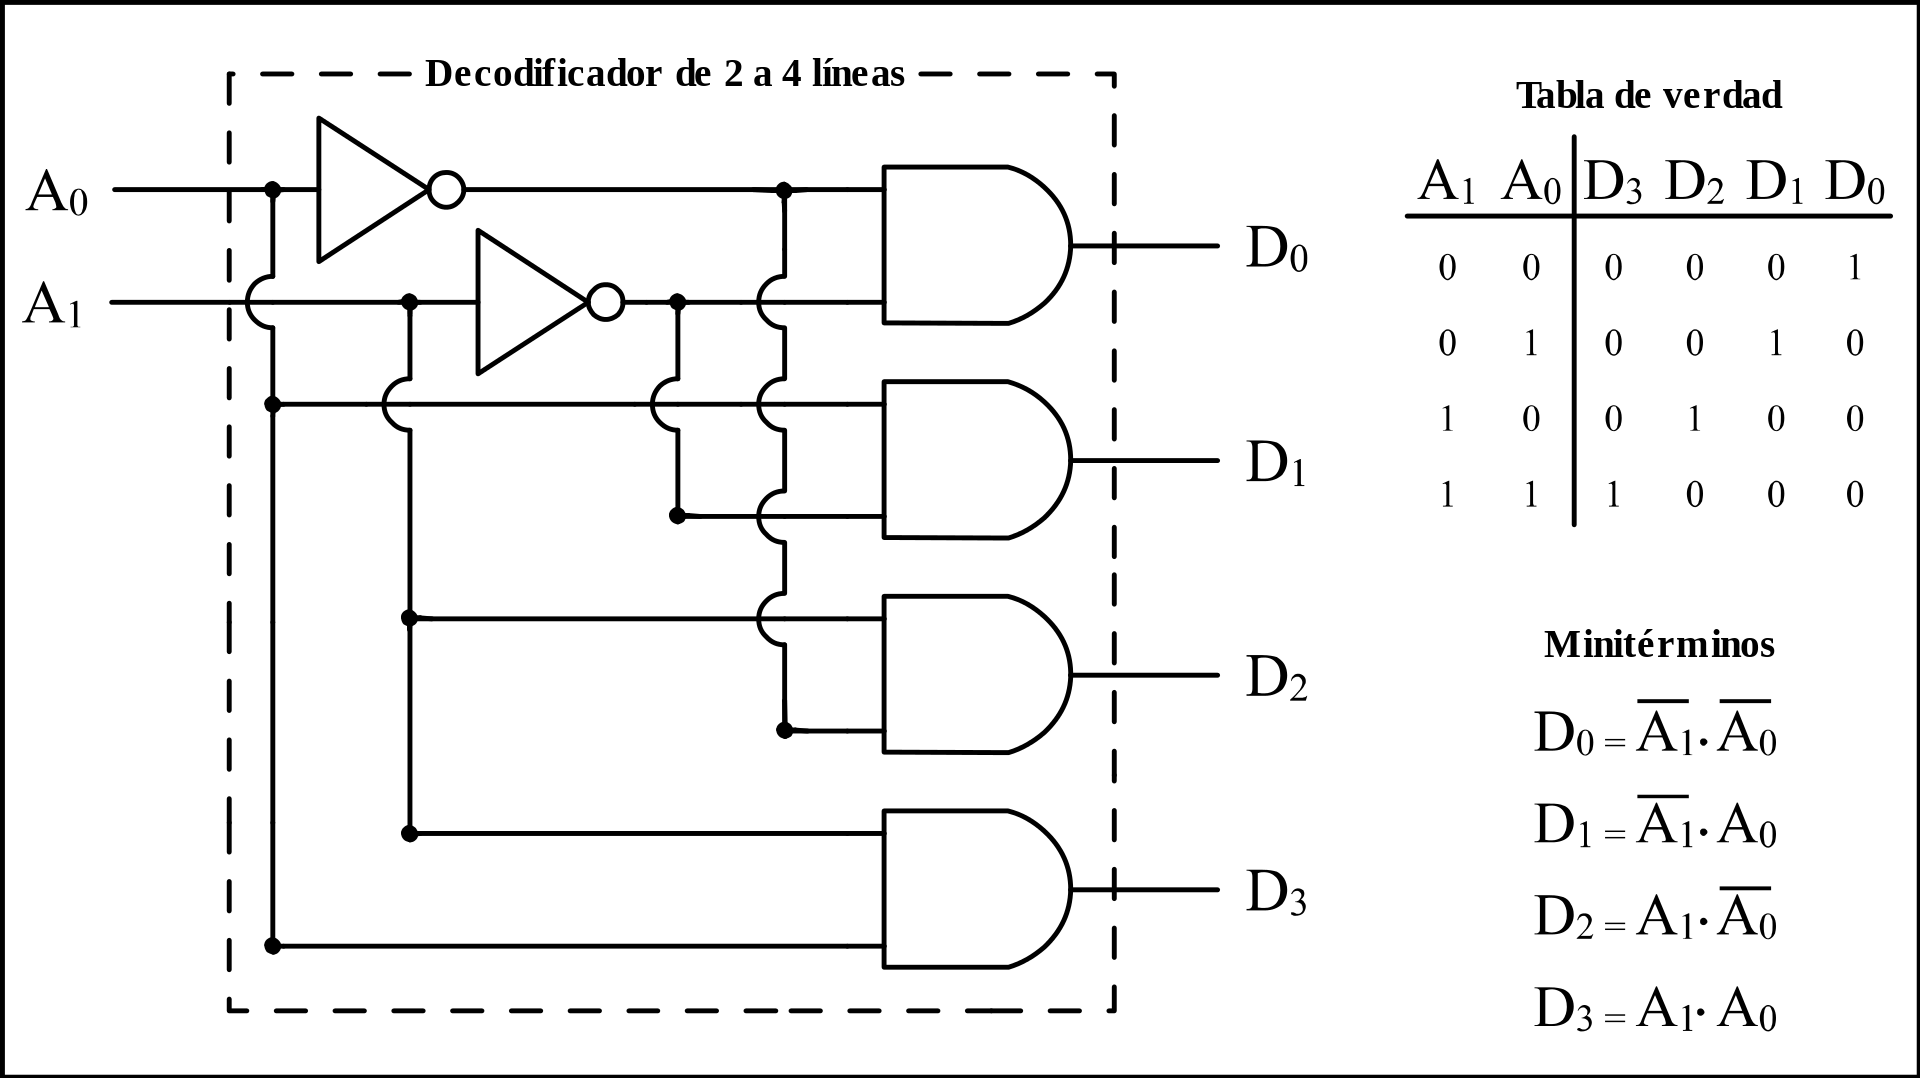
\includegraphics[width=0.7\linewidth]{Decoder_Example.png}
	\caption{Decodificador de código binario de dos bits a cuatro líneas de salida.  }
	\label{fig:decoderexample}
\end{figure}

Una posible implementación para Arduino de este decodificador es la siguiente.

\begin{lstlisting}[language=Arduino,numbers=none, showstringspaces=false]
	byte  DECO (bool A0, bool A1)
	{
		int i=0;
		bool D[4]={false, false, false, false};
		byte deco=0;
	
		D[0]=!A1 && !A0;
		D[1]=!A1 && A0;
		D[2]=A1 && !A0;
		D[3]=A1 && A0;
	
		for (i=0; i<sizeof(D);i++)
		{
			bitWrite(deco, i, D[i]);
		}
	return deco;
	}
\end{lstlisting}
  
\section{Lógica cableada}

El control eléctrico de motores es un conjunto de técnicas y dispositivos utilizados para administrar la operación de un motor eléctrico. El control eléctrico de motores se utiliza, para regular la velocidad, el par, la dirección de rotación, el arranque y el frenado del motor.

En general, el control eléctrico de motores implica la utilización de circuitos electrónicos y sistemas de control para ajustar el suministro de energía eléctrica al motor y así lograr la operación deseada. El control eléctrico de motores se aplica en una amplia gama de aplicaciones, desde equipos de producción industrial hasta electrodomésticos y sistemas de transporte.

\subsection{Contactor y relevador térmico}

Un contactor es un dispositivo electromecánico utilizado para controlar la conexión y desconexión de motores eléctricos u otros equipos eléctricos de alta potencia como; calentadores eléctricos, luminarias, banco de capacitores, etc. Los contactores consisten en un electroimán que activa los contactos eléctricos para permitir o interrumpir el flujo de corriente eléctrica hacia el motor, un ejemplo de un contactor de uso general se muestra en la Figura \ref{fig:contactor}. Los contactores suelen utilizarse en combinación con los relés de sobrecarga.


\begin{figure}
	\centering
	\begin{subfigure}[b]{0.4\textwidth}
		\centering
		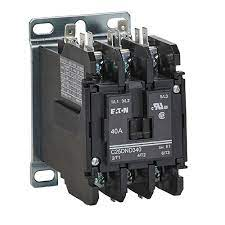
\includegraphics[width=\textwidth]{Contactor}
		\caption{Contactor de proposito general Eaton \cite{Eaton1}.}
		\label{fig:contactor}
	\end{subfigure}
\hfill
	\begin{subfigure}[b]{0.4\textwidth}
		\centering
		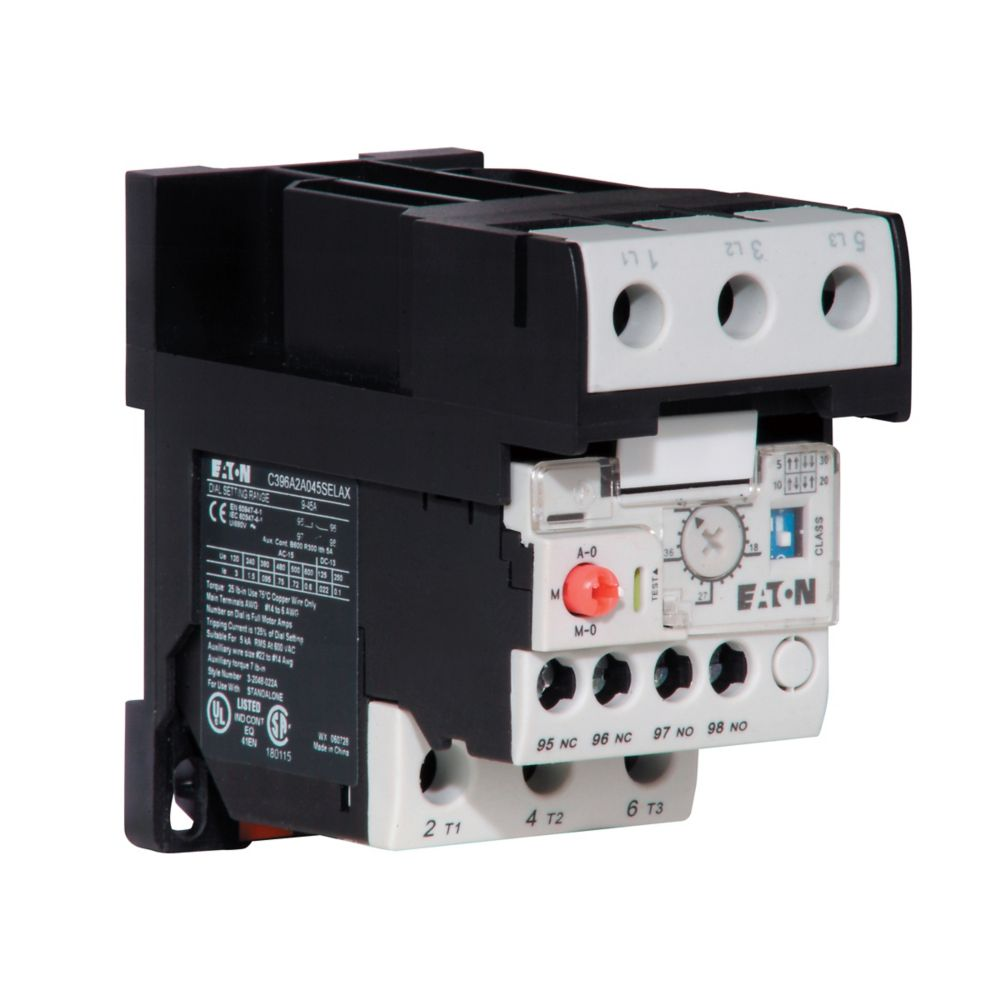
\includegraphics[width=\textwidth]{relevador}
		\caption{Relé de protección térmica Eaton \cite{Eaton2}.}
		\label{fig:rele}
	\end{subfigure}
\caption{Elementos de control y protección de motores.}
\end{figure}


Un relé de sobrecarga es un dispositivo de protección utilizado para evitar el sobrecalentamiento del motor eléctrico; la Figura \ref{fig:rele} muestra un relé de sobrecarga electrónico. Estos se clasifican en dos grandes tipos: Los térmicos y los electrónicos. Los relés térmicos detectan el aumento de temperatura del motor y, si la temperatura excede un cierto umbral, desconectan el motor para evitar daños. Los relés térmicos funcionan mediante el uso de elementos de medición de temperatura, como fusibles de alección eutéctica o bimetálicos, que desconectan los contactos del relé en caso de sobrecalentamiento.

Por otra parte los relés electrónicos posee una electrónica auto-alimentada con termistores que posee las siguientes características: poseen disparo ajustables para una protección óptima en diferentes condiciones de arranque, detectan  perdida de fase y desbalance, poseen liberación automática/manual para un rápido reinicio del proceso para una mayor disponibilidad, poseen una sensibilidad monofásica ajustable para cargas simétricas y asimétricas, detección integrada de la corriente de defecto a tierra en algunos casos y no requieren compensación térmica como los elementos térmicos. 


En conjunto, el contactor y el relé térmico se le llama arrancador electromagnético y se utilizan comúnmente en el control eléctrico de motores para proporcionar una interrupción segura y eficiente. Cuando se utiliza un contactor y un relé térmico en combinación, el contactor controla la conexión y desconexión del motor, mientras que el relé térmico proporciona protección contra  el sobrecalentamiento del motor.

\subsection{Curvas de disparo}

Las curvas clase 10, 20 y 30 son curvas de tiempo de disparo utilizadas en los elementos térmicos del relés según la norma NEMA (National Electrical Manufacturers Association) para la protección de motores eléctricos, ver Figura \ref{fig:curvasclass}.

Cada curva indica el tiempo tiempo de apertura del circuito  en función de la corriente de sobrecarga. La norma NEMA especifica los valores de corriente para cada curva son:

Curva clase 10: Esta curva se dispara en un tiempo de 10 segundos a una corriente de sobrecarga igual a 600\% de la corriente nominal del motor.

Curva clase 20: Esta curva se dispara en un tiempo de 20 segundos a una corriente de sobrecarga igual a 600\% de la corriente nominal del motor.

Curva clase 30: Esta curva se dispara en un tiempo de 30 segundos a una corriente de sobrecarga igual a 600\% de la corriente nominal del motor.

Es importante tener en cuenta que estas curvas de tiempo de disparo son solo una guía para la selección de los elementos térmicos, y la selección final dependerá de las características específicas del motor y la aplicación. Adicionalmente es importante que exista un correcta coordinación con el dispositivo de protección contra corto-circuito (SCPD) o breaker. La Figura \ref{fig:cordinacion} muestra el comportamiento de la corriente de un motor, la curva de protección térmica, la curva del SCPF y la curva que define la zona en que el motor se daña.

\begin{figure}
	\centering
	\begin{subfigure}[b]{0.48\textwidth}
		\centering
	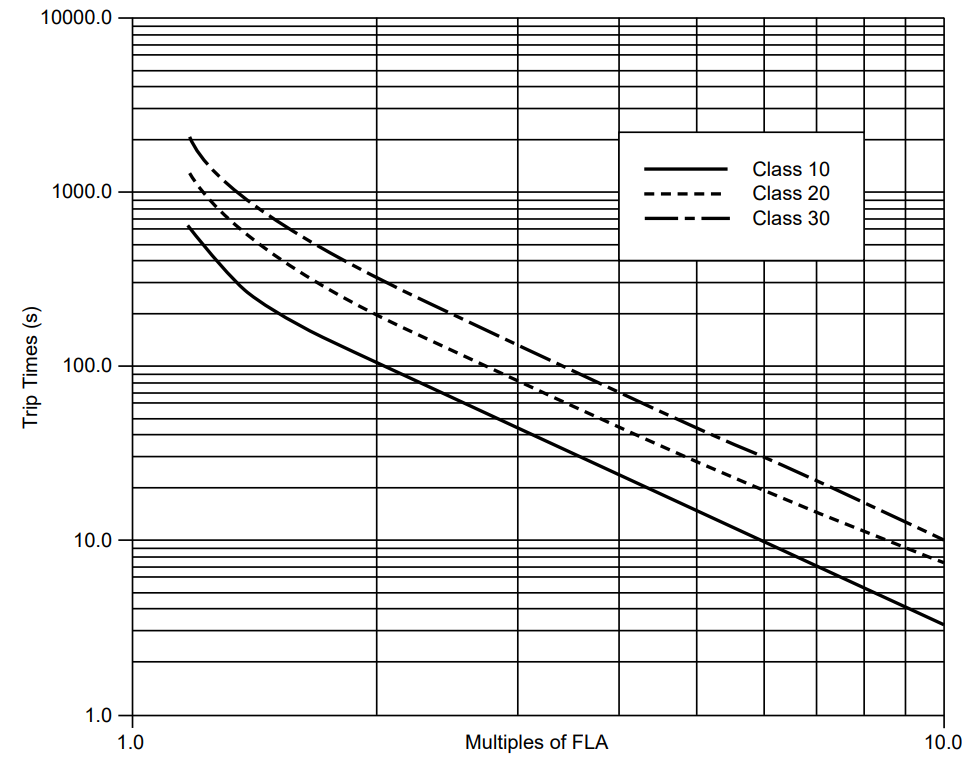
\includegraphics[width=\textwidth]{CurvasClass}
	\caption{Curvas NEMA Clase 10 , 20 , 30.}
	\label{fig:curvasclass}
	\end{subfigure}
	\hfill
	\begin{subfigure}[b]{0.5\textwidth}
		\centering
		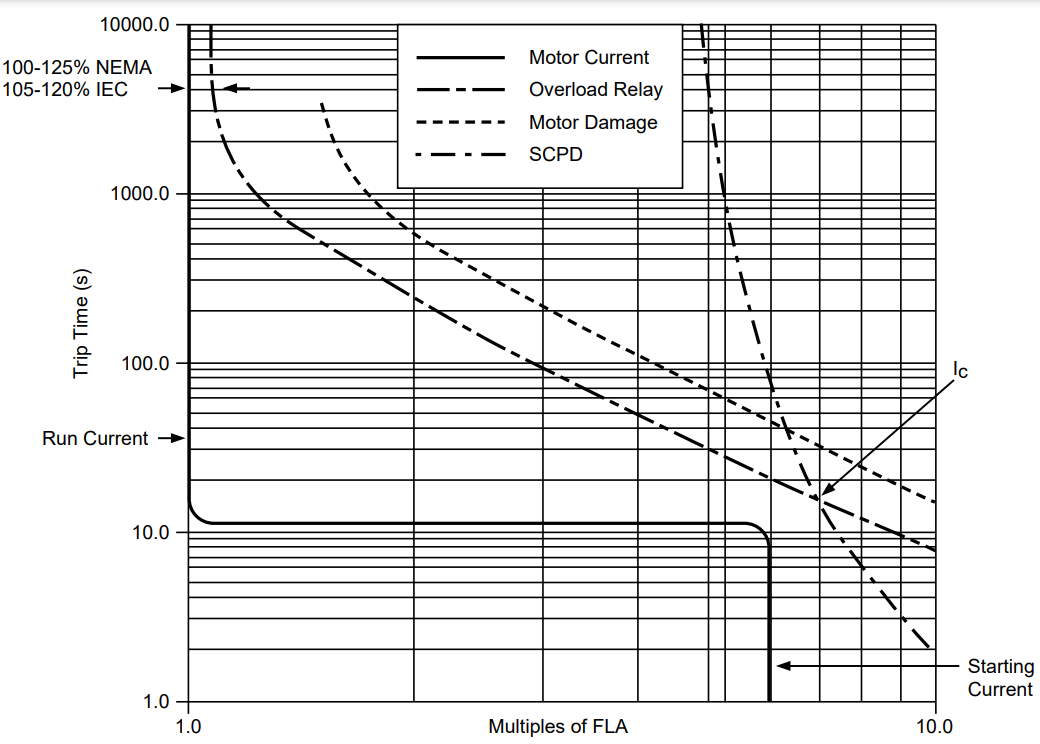
\includegraphics[width=\textwidth]{Cordinación}
		\caption{Coordinacion de curvas y zona de daño del motor.}
		\label{fig:cordinacion}
	\end{subfigure}
	\caption{Curvas de protección térmica \cite{Scheneider}.}
\end{figure}


\subsection{Selección de componentes}

Usualmente cada fabricante propone su procedimiento de selección para contactores o relevadores, sin embargo los procedimientos tienen criterios comunes. Usualmente los contactores se seleccionan por: potencial del motor, voltaje de línea, voltage de la bobina, frecuencia de la red, vida útil (o cantidad de operaciones mínima requerida) y tipo de protección ambiental que se requiera, esto último se refiere al tipo de gabinete donde se monta el contactor. 
Por otra parte, los relevadores se seleccionan según la corriente nominal, la aplicación determina el tiempo de disparo de la curva, el tamaño del contactor al que debe ser acoplado y la compensación ambiental sólo en relevadores térmicos.  


\section{Arranques a tensión reducida}
El arranque de motores trifásicos a tensión reducida es una técnica utilizada para reducir la corriente de arranque y el par de arranque, lo que ayuda a evitar problemas de sobrecarga en el sistema eléctrico.

Existen diferentes técnicas, pero las más comunes son: de arranque a tensión reducida, como el arranque estrella-triángulo, el arranque con autotransformador, arranque con resistencias estatóricas o rotóricas, arrancadores suaves, etc. Cada técnica tiene sus propias ventajas y desventajas y debe seleccionarse en función de las características del motor, la aplicación y las limitaciones del sistema eléctrico.

\subsection{Temporizadores Electrónicos}

Los temporizadores son dispositivos de control de tiempo que permiten activar o desactivar algún actuador un tiempo después de activarse o desactivarse una señal de control. Los temperorizadores pueden ser  construidos de forma mecánica, neumática, electromecánica, electrónica, programada pero todos tienen funcionamientos estandarizados como: retardo a la conexión (On-delay), retardo a la desconexión (Off-delay), retardo a la conexión y desconexión (On/Off-Delay), relés de pulsos simétricos, entre otros. 

La Figura \ref{fig:imagen} muestra un temporizador electrónico y la Figura \ref{fig:Diagrama} su diagrama de conexión. Note que el dispositivo se alimenta mediante las borneras A1-A2,  las señales de control se declaran como X1 y Y1, y los contactos auxiliares normalmente cerrados y abiertos son las borneras 15-16-18 y 21-22-24. Este temporizador posee cuatro potenciometros o diales: el  primer dial selecciona el rango de tiempo $R$, con el segundo dial se selecciona un valor $V$ entre 1 y 10, el tiempo de activacion  $T$ se calcula como  $T=R\cdot V/10$. El tercer dial selecciona una de las ocho funciones preestablecidas: a modo de ejemplo la Figura \ref{fig:Funciones} muestra las funciones A, C, Ac que representan temporizador operando como: On-delay, Off-delay y On-Off delay. Finalmente el cuarto dial, permite establecer un tiempo de retardo entre los contactos auxiliares R1 y R2, más información se detalla en \cite{Scheneider4}.


\begin{figure}
	\centering
	\begin{subfigure}[b]{0.3\textwidth}
		\centering
		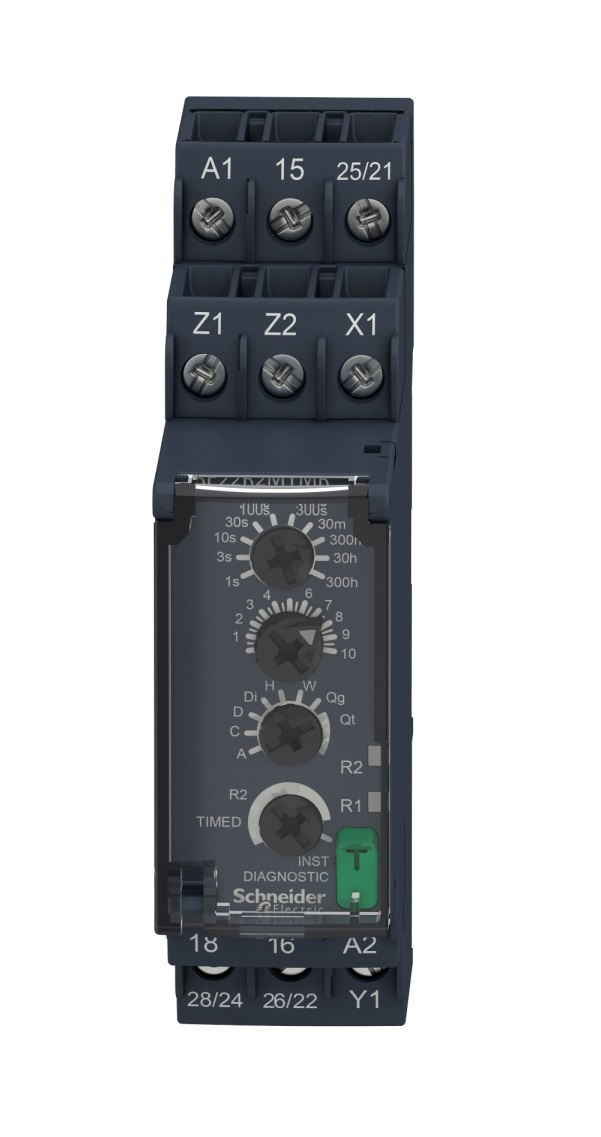
\includegraphics[width=\textwidth]{RE22R2MYMR}
		\caption{Temporizador RE22R2MYMR \cite{Scheneider3} }
		\label{fig:imagen}
	\end{subfigure}
	\hfill
	\begin{subfigure}[b]{0.5\textwidth}
		\centering
		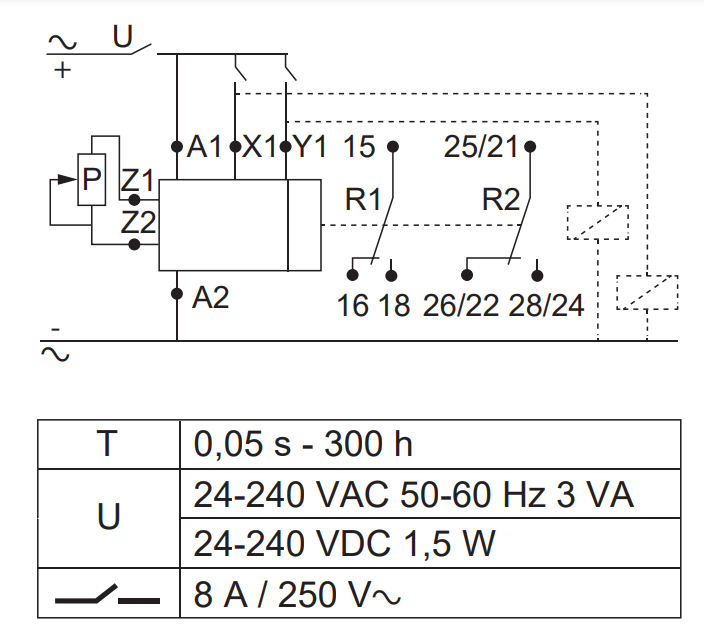
\includegraphics[width=\textwidth]{TimerDiagram}
		\caption{Diagrama de conexión del RE22R2MYMR \cite{Scheneider4} }
		\label{fig:Diagrama}
	\end{subfigure}
	\caption{Temporizador de 8 funciones RE22R2MYMR.}
\end{figure}



\begin{figure}
	\centering
	\begin{subfigure}[b]{0.32\textwidth}
		\centering
		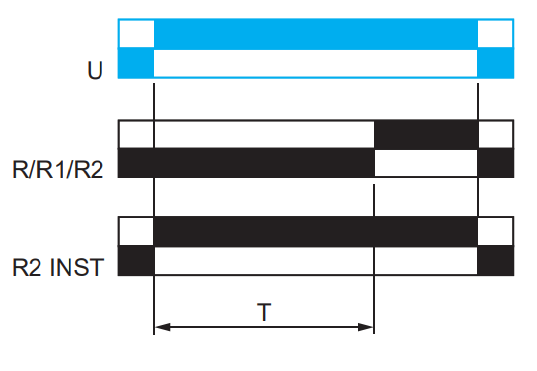
\includegraphics[width=\textwidth]{A-OnDelay}
		\caption{A: On delay }
		\label{fig:on-delay}
	\end{subfigure}
	\begin{subfigure}[b]{0.32\textwidth}
		\centering
		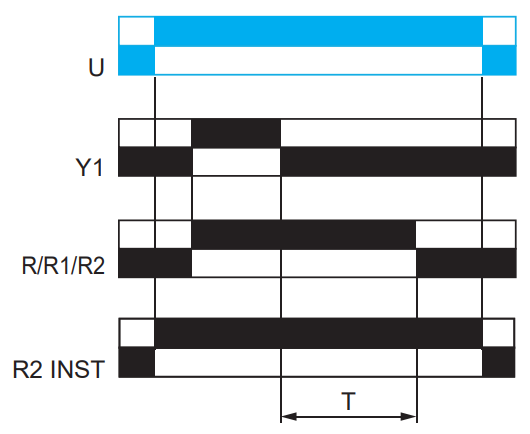
\includegraphics[width=\textwidth]{C-OffDelay}
		\caption{C: Off delay}
		\label{fig:Off-delay}
	\end{subfigure}
	\begin{subfigure}[b]{0.32\textwidth}
	\centering
	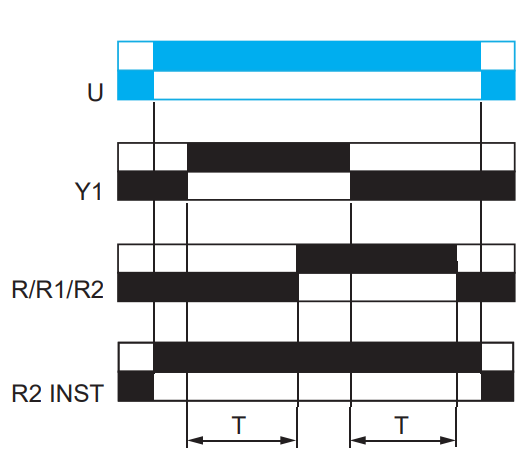
\includegraphics[width=\textwidth]{Ac-On-OffDelay}
	\caption{Ac: On-Off delay }
	\label{fig:OnOff-delay}
	\end{subfigure}
	\caption{Diagramas de tiempo de funciones a escoger en el selector del temporizador \cite{Scheneider4}.}
	\label{fig:Funciones}
\end{figure}

\section{Variadores de frecuencia}


Los arrancadores suaves son sistemas electrónicos de control de motores que permiten arrancar y parar motores asíncronos de inducción. Los arrancadores suaves disponen de dos tiristores conectados en antiparalelo en dos de las tres fases como se muestra en la Figura \ref{fig:controlfase}. La corriente en la tercera fase no controlada, es una suma de las corrientes de las dos fases controladas. El arrancador suave realiza un recorte del angulo $\alpha$ en cada fase, por lo tanto, la tensión del motor aumenta desde un voltaje inicial hasta la tensión a plena carga en un tiempo definido por el usuario. La tensión de inicio y el tiempo de la rampa se relacionan según la Figura \ref{fig:rampasarrancador} y estos parámetros son ajustados mediante los dos potenciometros de la Figura \ref{fig:3rw3013-1bb14gic03xx31074p} .

La intensidad del motor tiene un comportamiento proporcional a la tensión aplicada al motor. De este modo, la corriente de arranque se reduce en el mismo factor que la tensión aplicada al motor. La Figura \ref{fig:corrientemotor} muestra la reducción en la corrientes. Por otra parte, el torque tiene un comportamiento cuadrático respecto a la tensión aplicada al motor. La Figura \ref{fig:torquemotor} muestra como el par de arranque se reduce de forma cuadrática con la tensión aplicada al motor. En ambos casos se aprecia las curvas de corrientes y torque con rampas de tiempo cortas o prolongadas.

\begin{figure}
	\centering
	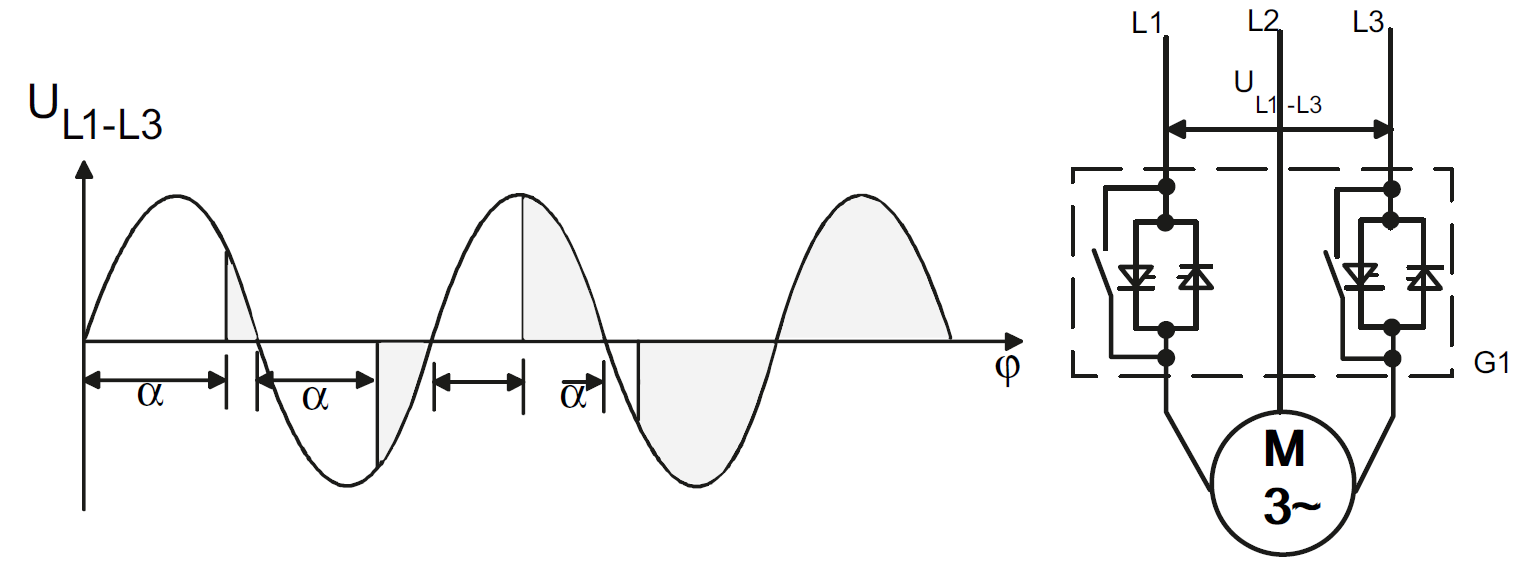
\includegraphics[width=0.75\linewidth]{ControlFase}
	\caption{Control por recorte de fase y esquema de un arrancador suave con control bifásico. \cite{SIEMENS}}
	\label{fig:controlfase}
\end{figure}



\begin{figure}
	\centering
	\begin{subfigure}[b]{0.69\textwidth}
		\centering
		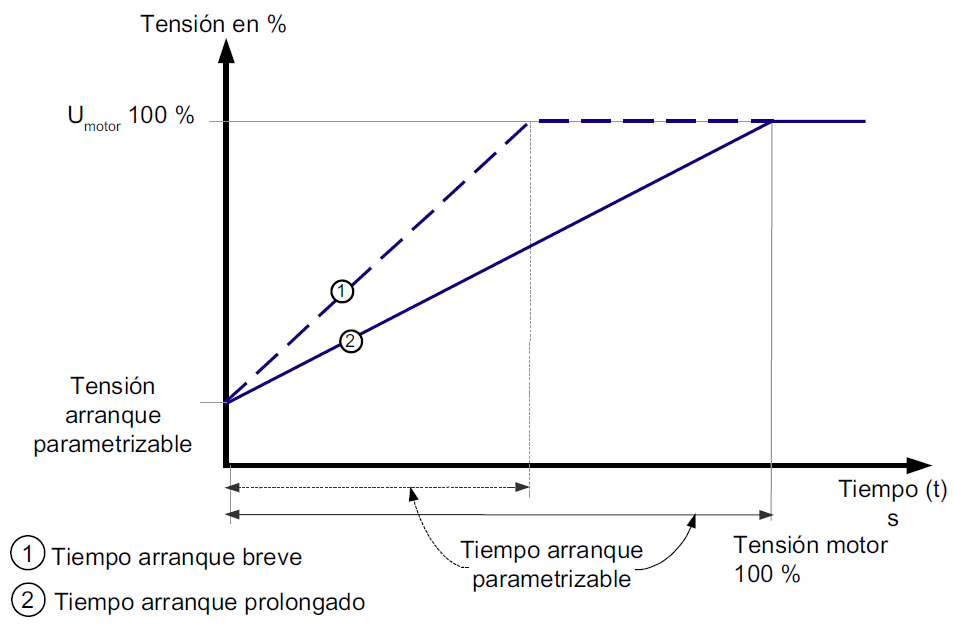
\includegraphics[width=\textwidth]{RampasArrancador}
		\caption{Principio de funcionamiento}
		\label{fig:rampasarrancador}
	\end{subfigure}
	\hfill
	\begin{subfigure}[b]{0.3\textwidth}
		\centering
		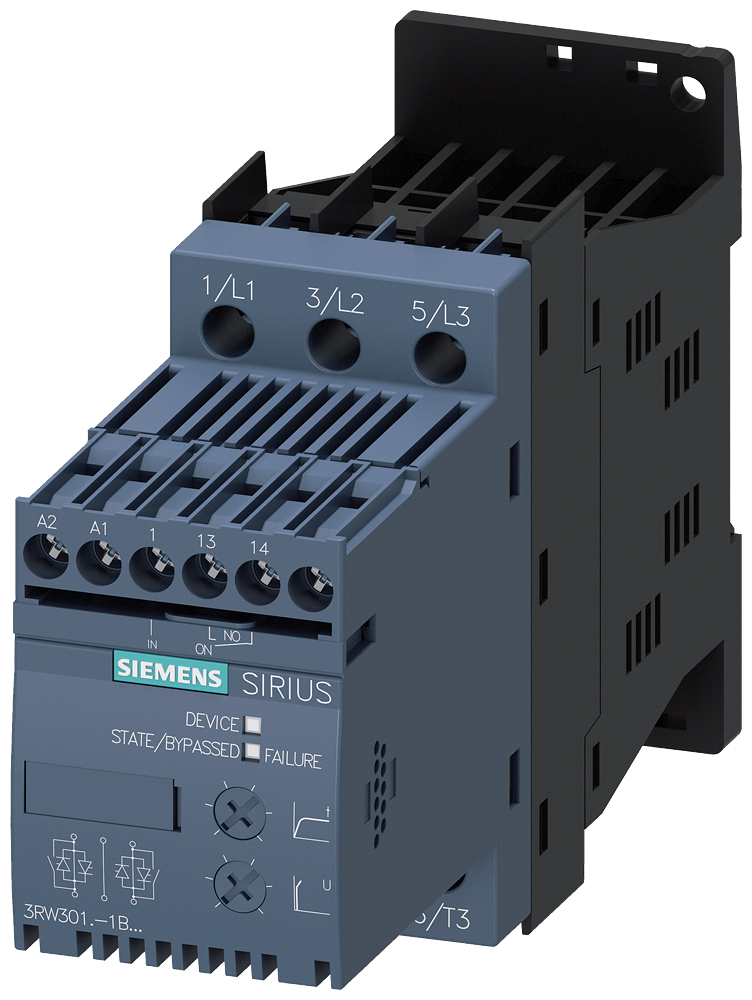
\includegraphics[width=\textwidth]{3RW3013-1BB14_G_IC03_XX_31074P}
		\caption{Imagen del arrancador}
		\label{fig:3rw3013-1bb14gic03xx31074p}
		
	\end{subfigure}
	\caption{Arrancador suave SIEMENS 3RW3013.\cite{SIEMENS}}
\end{figure}


\begin{figure}
	\centering
	\begin{subfigure}[b]{0.49\textwidth}
		\centering
		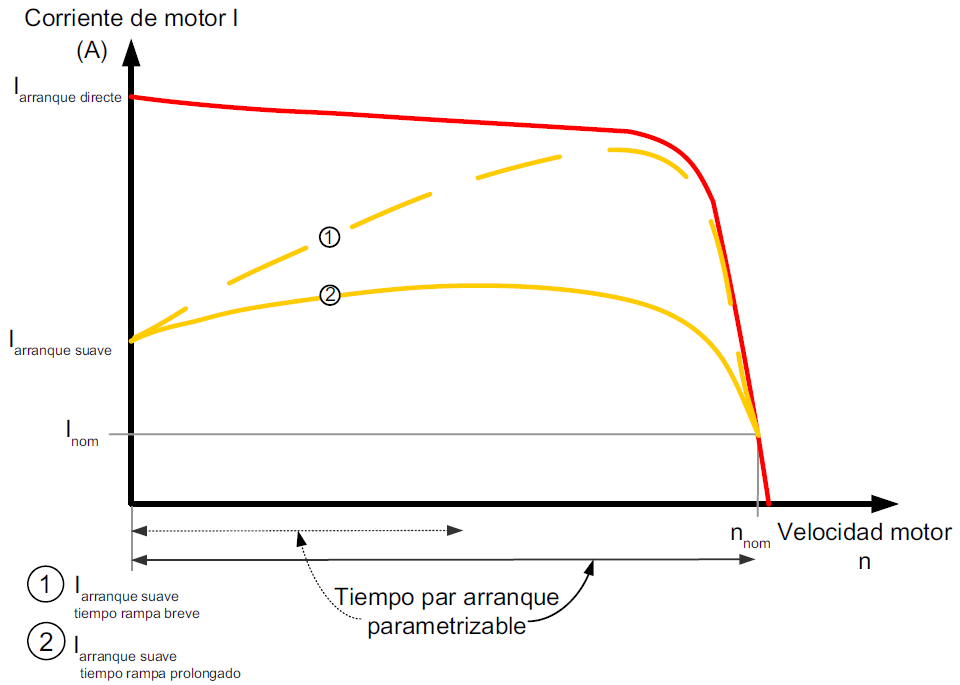
\includegraphics[width=\textwidth]{CorrienteMotor}
		\caption{Corrientes del motor}
		\label{fig:corrientemotor}
	\end{subfigure}
	\hfill
	\begin{subfigure}[b]{0.49\textwidth}
		\centering
		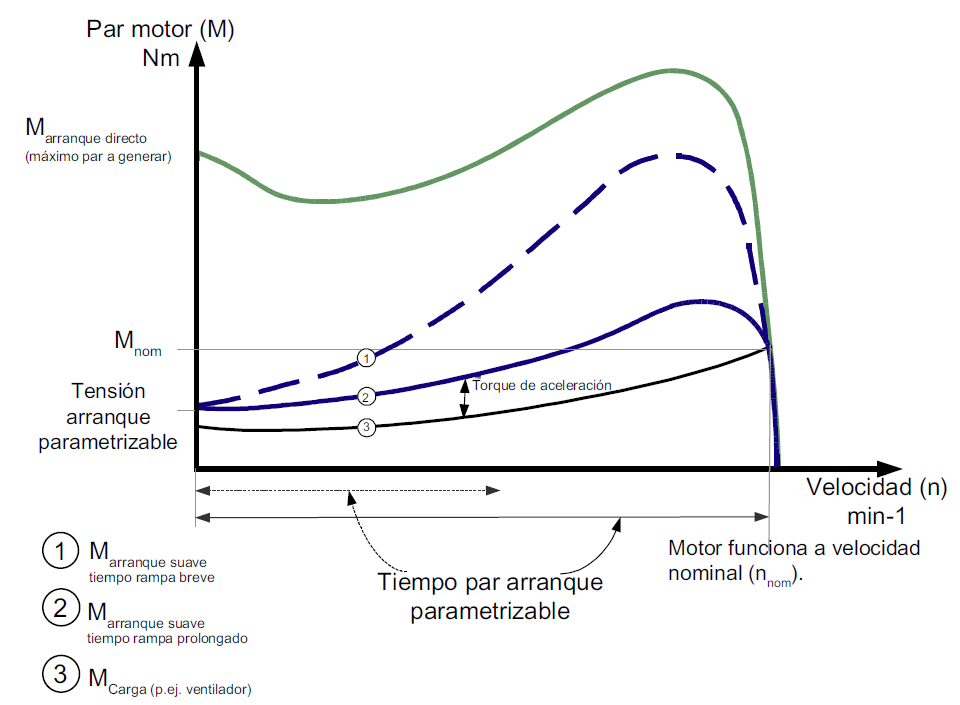
\includegraphics[width=\textwidth]{TorqueMotor}
		\caption{Torque del motor}
		\label{fig:torquemotor}
		
	\end{subfigure}
	\caption{Curvas de corrientes y torques versus velocidad.\cite{SIEMENS}}
\end{figure}

\subsection{Variadores de Frecuencia}

Un variador de frecuencia (VDF) es un dispositivo que se utiliza para controlar la velocidad y el par de un motor eléctrico alterando la frecuencia y el voltaje suministrado al mismo. El VDF es capaz de convertir la corriente alterna (CA) de entrada, en una señal de pulsos alternos con frecuencia y voltaje adecuados para el motor. Esta señal de salida se llamada modulación por ancho de pulso (PWM). La Figura \ref{fig:pwm} muestra señales PWM que equivalentes a señales sinosoidales de: a) 60 Hz y 120V, b)30Hz y 60V, c) 20Hz y 40V.

\begin{figure}
	\centering
	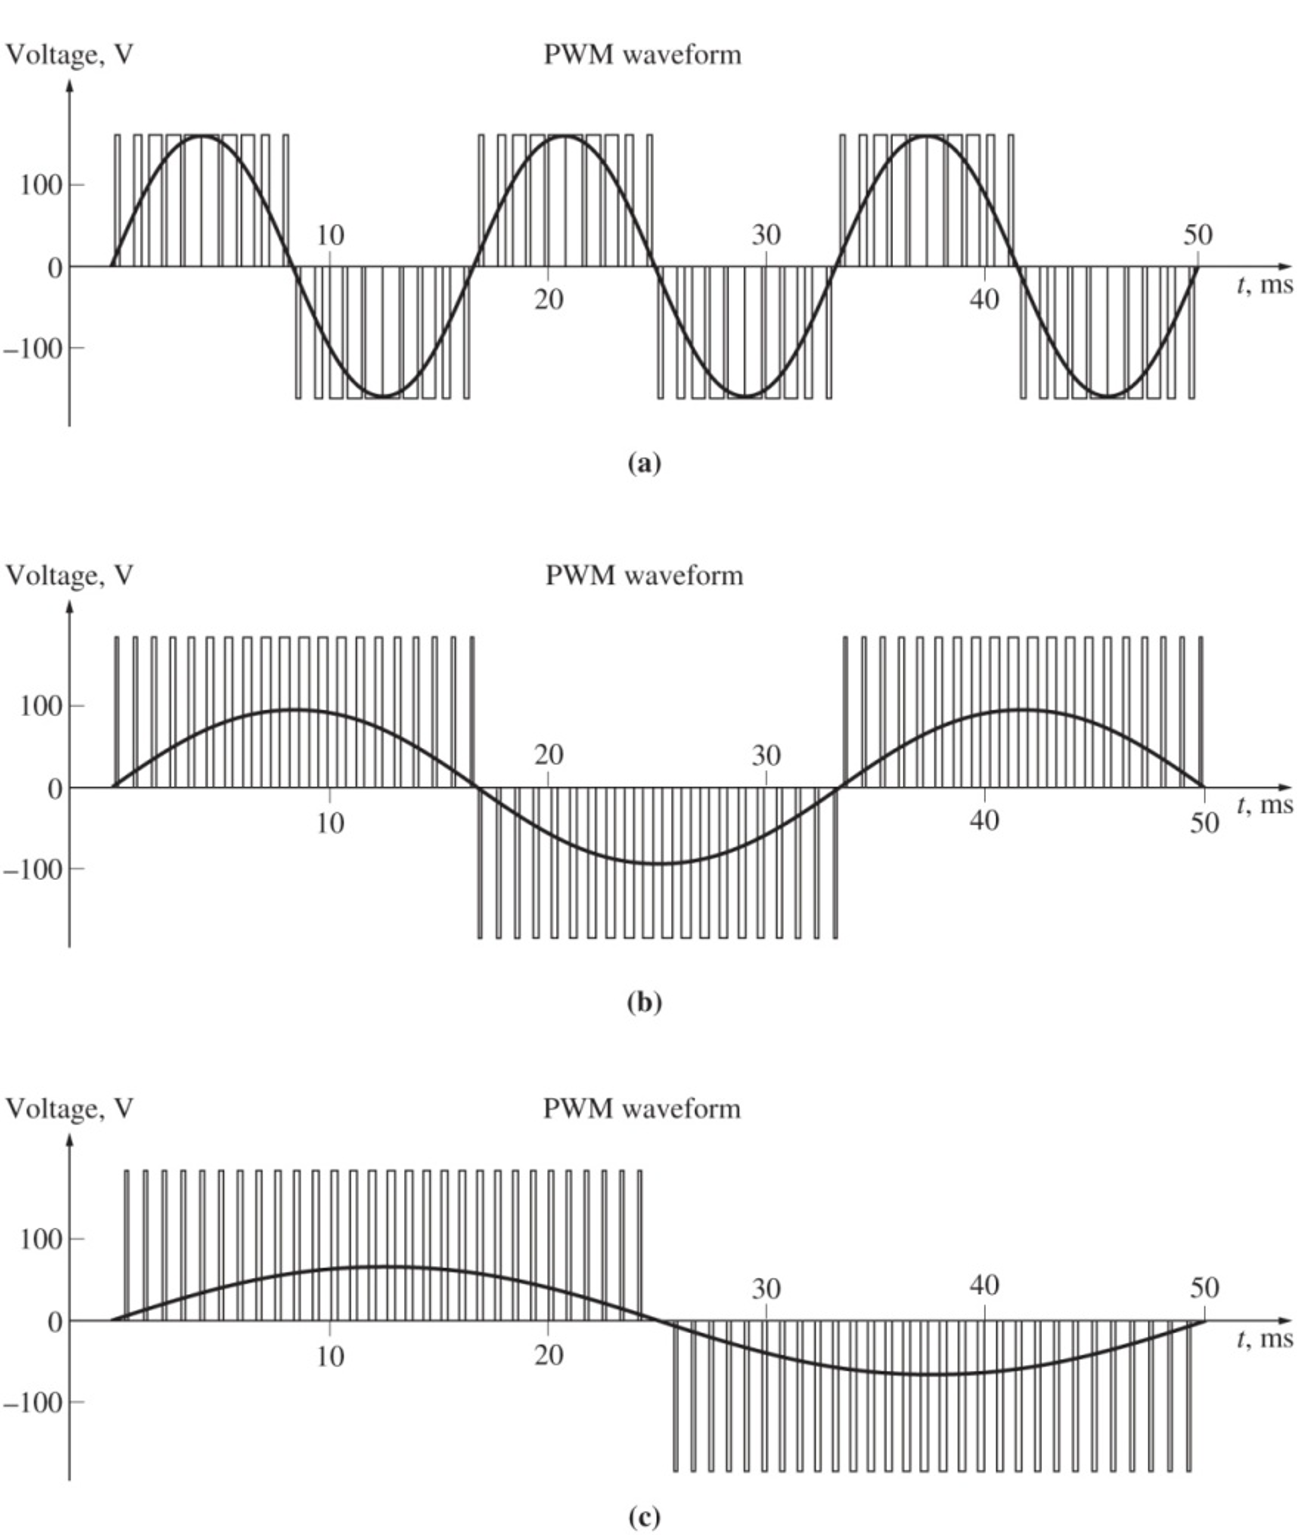
\includegraphics[width=0.8\linewidth]{pwm2}
	\caption{Señales PWM equivalentes a señales sinosoidales de distintas amplitud y frecuencia \cite{Chapman12}.}
	\label{fig:pwm}
\end{figure}


El variador de frecuencia permite variar la velocidad del motor eléctrico en función de las necesidades de la aplicación, lo que puede resultar en un ahorro de energía y un mayor control de la velocidad. Además, el variador de frecuencia también puede proporcionar protección al motor, ya que puede detectar y proteger contra situaciones de sobrecarga, cortocircuito y fallos de fase, entre otros problemas.

Un VDF puede operar bajo dos principios: el control escalar y control vectorial \cite{Posadas05}. El control escalar, también conocido como control $V/f$ (voltaje/frecuencia), es el método de control más simple y comúnmente utilizado en los variadores de frecuencia. En este método, se ajusta la frecuencia y el voltaje de salida del variador en función de la carga del motor para mantener una relación de flujo magnético constante equivalente a la relación $V/f$. El control escalar es más adecuado para aplicaciones que requieren un control de velocidad básico, como ventiladores y bombas. 

Por otra parte, el control vectorial, conocido como control de campo orientado, es una técnica de control avanzada que permite un mayor grado de precisión en el control del motor. En este método, se utiliza un modelo matemático del motor para controlar tanto la velocidad como el par del motor de manera independiente. Esto se logra mediante el control de la corriente y el voltaje en el estator del motor, lo que permite un control preciso de la orientación del campo magnético del motor. El control vectorial es más adecuado para aplicaciones que requieren un control de velocidad preciso y una alta dinámica, como en máquinas herramienta y robots industriales.

\subsection{Partes del variador}

La Figura \ref{fig:ab160} muestra las principales partes del VDF y se detallan a continuación:
\begin{enumerate}
	\item Rectificador: Es la parte que convierte la energía eléctrica de entrada en una señal de corriente directa (CD) que se utiliza como entrada para el inversor.
	
	\item Inversor: Es la parte que convierte la señal de corriente directa (CD) en una señal PWM con la frecuencia y el voltaje adecuados para el motor.
	
	\item Microprocesador: Es el cerebro del variador y controla todas las funciones y operaciones del mismo. El microprocesador recibe las señales de entrada y, en función de los parámetros de programación establecidos, envía las señales adecuadas al rectificador e inversor para controlar la velocidad y el par del motor.
	Adicionalmente el controlador se encarga de monitorear el variador, incluyendo la protección del motor contra sobrecargas, cortocircuitos, fallos de fase, etc.
	
	\item Interfaz de usuario: Es la parte que permite a los usuarios interactuar con el variador, configurar los parámetros de programación y monitorear su operación.
	
	\item Circuitos de medición: son los circuitos encargados de medir las variables eléctricas del variador y el motor, incluyendo la protección del motor contra sobrecargas, cortocircuitos, fallos de fase, etc.
	
\end{enumerate}

\begin{figure}
	\centering
	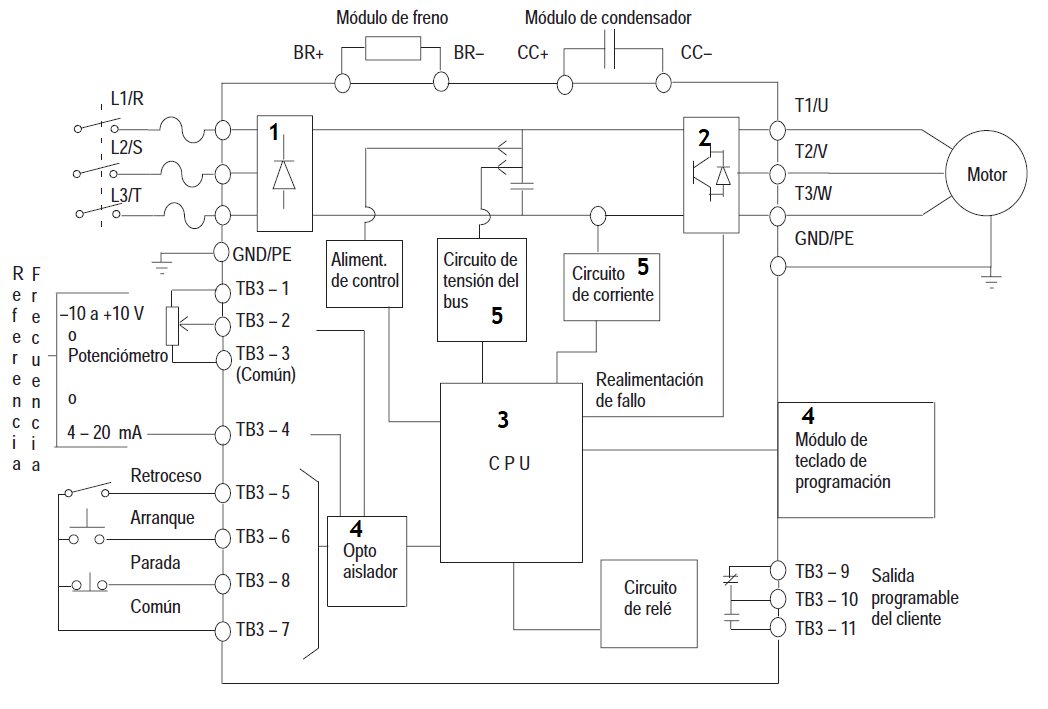
\includegraphics[width=0.9\linewidth]{AB160}
	\caption{Esquema del Variador de Frecuencia AB160.\cite{AB160} }
	\label{fig:ab160}
\end{figure}

\subsection{Parámetros de programación}

 Los parámetros para configurar un VDF puede oscilar desde unos pocos parámetros básicos hasta cientos. Sin embargo los obligatorios son definidos por la red eléctrica, los datos de placa del motor y la aplicación. Entre ellos destaca: Tensión base o tensión nominal del motor, Frecuencia nominal del motor, frecuencia mínima y máxima de operación del motor,  modos de parada del motor , modos de entrada (cableado de entrada), modos de salida (relés de alarmas), tiempo de aceleración y desaceleración del motor y frecuencias restablecidas activadas por señales digitales.
 
Para el calculo de los  tiempos de aceleración y desaceleración se requiere conocer el torque del motor ($T_m$), el torque de la carga ($T_r$), la inercia total del sistema mecánico $J$, la velocidad angular  de inicio ($\omega_i$),  la velocidad angular final ($\omega_f$) y el delta de tiempo ($\Delta t$) que es el tiempo que se tarda entre ambas velocidades angulares. Por lo tanto el torque de aceleración ($T_A$) debe ser siempre menor al $150\% T_m$ de lo contrario existirán problemas de sobrecarga.

\begin{equation}
T_A=J\dfrac{(\omega_f-\omega_i)}{\Delta t} + T_r
\end{equation}

Si se asume que un motor de inducción  puede entregar un torque máximo de 150\% de su torque, entonces  las rampas de aceleración se calculan como:

\begin{equation}
\Delta t=J\dfrac{(\omega_f-\omega_i)}{1.5 T_m-T_r}
\end{equation}
 
 El tiempo natural en que se frena la inercia esta dado por \eqref{Eq:Tmin}, si se requiere frenar el sistema de forma más acelerada, es necesario colocar en el VDF resistencias que disipan la potencia eléctrica entregada por el motor, el cual se encuentra operando como alternador.
 
 \begin{equation}
 \Delta t=J\dfrac{\omega_i}{T_r}
 \label{Eq:Tmin}
 \end{equation}
 
 Por otra parte, la frecuencia de operación del VDF se selecciona según las necesidades mecánicas de la carga; por ejemplo, el motor de un reductor de velocidad debe operar a 950 revoluciones por minuto (rpm). Para determinar la frecuencia  que se debe programar, se requiere conocer el deslizamiento del motor ($s$), sus polos ($p$), la frecuencia nominal ($f_n$), el tipo o comportamiento de la carga (torques constantes, torques variables).
 
 Cuando el torque de la carga es constante, Figura \ref{fig:torqueconstante}, las velocidades de deslizamiento son contantes no importa la frecuencia en que opera el motor. Esto implica que el deslizamiento en el nuevo punto de operación($s_2$) está dado por, $s_2=s\cdot f_n/f_2$. Sabiendo que la velocidad mecánica está dada por:
 
 \begin{equation}
 	\eta_{mec}=\dfrac{120f_n}{p}(1-s)
\end{equation}
 entonces, la nueva frecuencia  ($f_2$) a programar el en VDF en función de la  velocidad mecánica deseada ($\eta_{mec2}$) se determina de la siguiente  forma,
 \begin{equation}
 f_2=\dfrac{p\left(\eta_{mec2}+ \dfrac{120sf_n}{p}\right) }{120}.
 \end{equation} 
 
 Las bombas centrifugas o abanicos  son ejemplos de par resistente variable, tal y como se aprecia en la figura \ref{fig:torquevariable}. En estos casos la velocidad de deslizamiento varia según la carga, pero una aproximación con error menor al 1\% asume que los deslizamientos son constantes, por tanto  $s_2=s$.
 
 
 \begin{figure}
 	\centering
 	\begin{subfigure}[b]{0.49\textwidth}
 		\centering
 		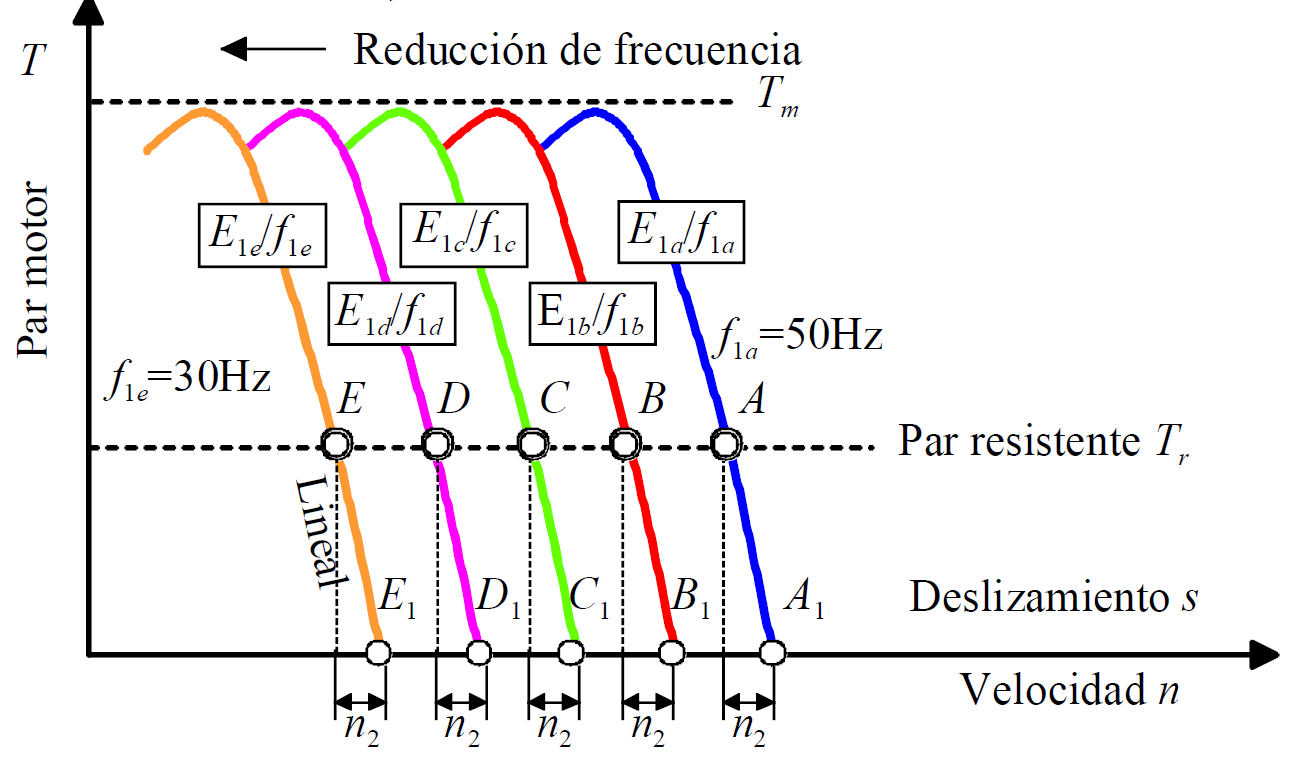
\includegraphics[width=\textwidth]{TorqueConstante}
 		\caption{Torque carga constante}
 		\label{fig:torqueconstante}
 	\end{subfigure}
 	\hfill
 	\begin{subfigure}[b]{0.49\textwidth}
 		\centering
 		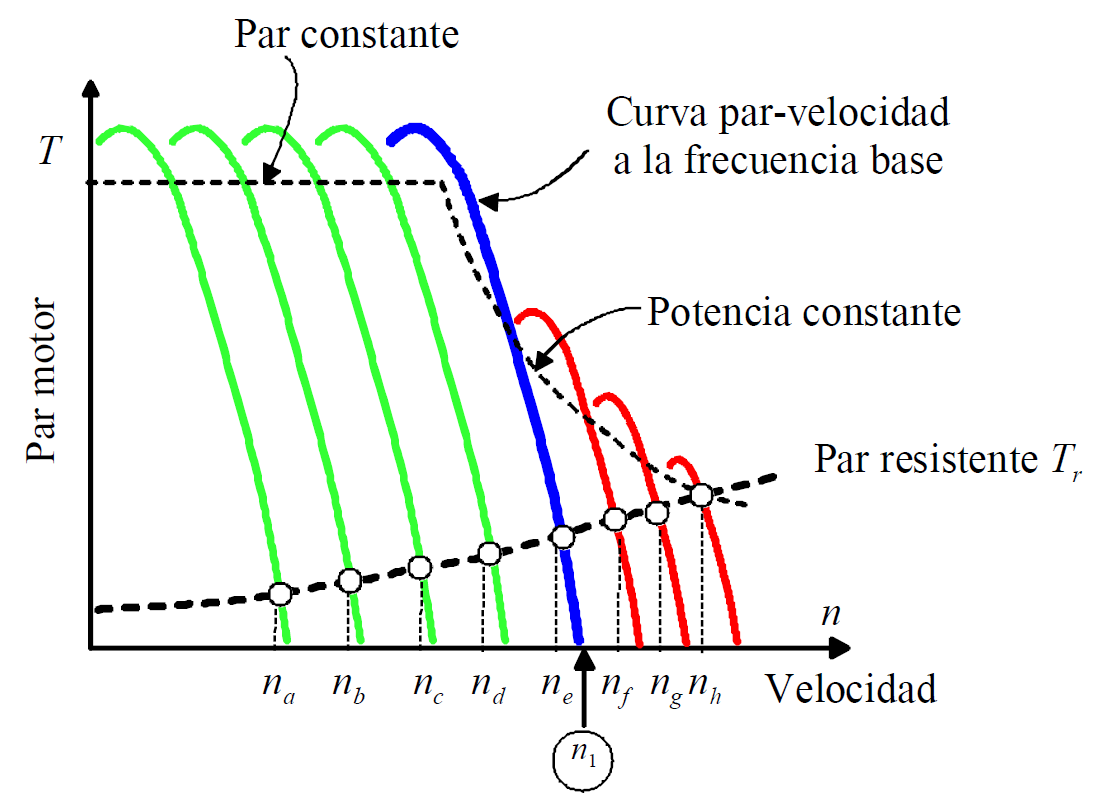
\includegraphics[width=\textwidth]{TorqueVariable}
 		\caption{Torque de carga variable}
 		\label{fig:torquevariable}
 	\end{subfigure}
 	\caption{Curvas de torque inducido del motor y par de la carga. \cite{Mora08}}
 \end{figure}
 

 \section{Logo!}

Como se indica en el manual \cite{LOGO1}, el LOGO! un módulo lógico universal para el control de procesos industriales o automatización, que incorpora funciones lógicas, temporizadores, contadores, controladores PID, funciones aritméticas, fuente de alimentación, interfaces gráficas, módulos de ampliación y el software de programación. La figura muestra un LOGO!8 24CE, de 24 voltios y salidas a transistor.
\begin{figure}
	\centering
	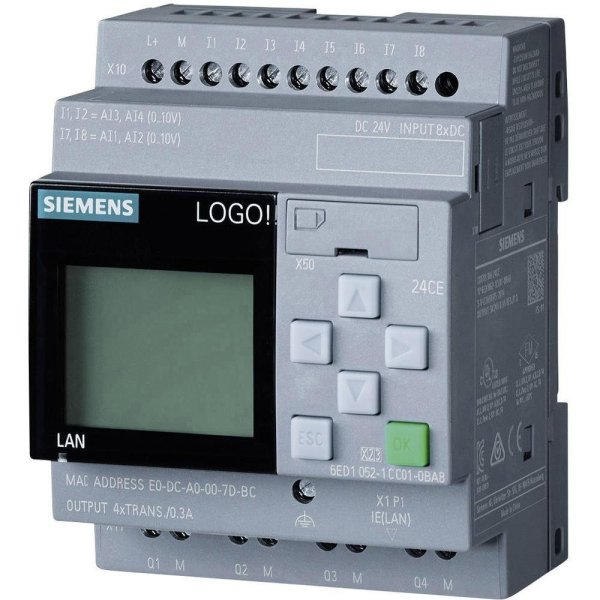
\includegraphics[width=0.5\linewidth]{Logo!8.jpg}
	\caption{LOGO!8 24CE.}
	\label{fig:logo8}
\end{figure}

 El alambrado del dispositivo esta explicado en la sección 2.3 del Manual del LOGO! \cite{LOGO1}. Hay que tener en cuenta que dependiendo del modelo del LOGO, la forma de como se alambra la alimentación, las señales de entradas y las señales de salida podrían cambiar. Respecto a la alimentación, es importante la colocación de fusibles o varistores (MOV) dependiendo del modelo, ver pagina 43 del manual.  Un ejemplo básico de un programa de control en LOGO, con el alambrado físico se muestran en la sección 3.3 del manual \cite{LOGO1}.
 
 El LOGO es programado con el software llamado \href{https://new.siemens.com/global/en/products/automation/systems/industrial/plc/logo/logo-software.html}{\textit{LOGO!Soft Comfort}}. En el manual del software \cite{LOGO2}, en el capítulo 3, página 164, se muestra un Tutorial del uso del programa. Por otra parte, dicho manual brinda los siguientes cinco ejemplos resueltos para su estudio:
 
\begin{itemize}
	\item Bomba de agua no potable (página 219).
	\item Sistema de ventilación (página 235).
	\item Portón corredizo (página 236).
	\item Control de calefacción (página 238).
	\item Estación de llenado (página 241).	
\end{itemize}
 
\section{Autómatas programables}

La programación de los autómatas programables ha sufrido cambios en la semántica y sintaxis de programación con la implementacion de la norma IEC 611131-3 \cite{IEC61131-1} por parte de los fabricantes. La normalización de la semántica  mediante la estructuración de los programas y la normalización de sintaxis mediante la implementacion de cinco lenguajes de programación estandarizados  permiten la portabilidad del código entre fabricantes. 

La programación  estructura de  código informático para autómatas programables, permite organizar y descomponer  las soluciones en multiples subsistemas con distintos niveles de jerarquía. Esta  nueva forma de programar estructuradamente permite ordenar y dar mantenimiento al código de forma más sencilla, así como re-utilizar  código existente para otras soluciones. Al respecto la norma IEC-61131-3 \cite{Tiegelkamp10} indica que los autómatas modernos estructuran sus programas en \textit{Program Organisation Units} (POU) los cuales los divide en tres tipos: \textit{Program}, \textit{Function Block} y \textit{Funtion}.  

SIEMENS indica en su manual de Software \cite{TIA-S7}, que el programa de usuario se conforma por: bloques  de organización (OB), bloques de función (FB), funciones (FC), y bloques de datos (DB), la Figura \ref{fig:plc} muestra la relación entre los distintos bloques. Por favor leer entre las páginas 5625-5631 para una descripción detallada de los bloques.

\begin{figure}[H]
	\centering
	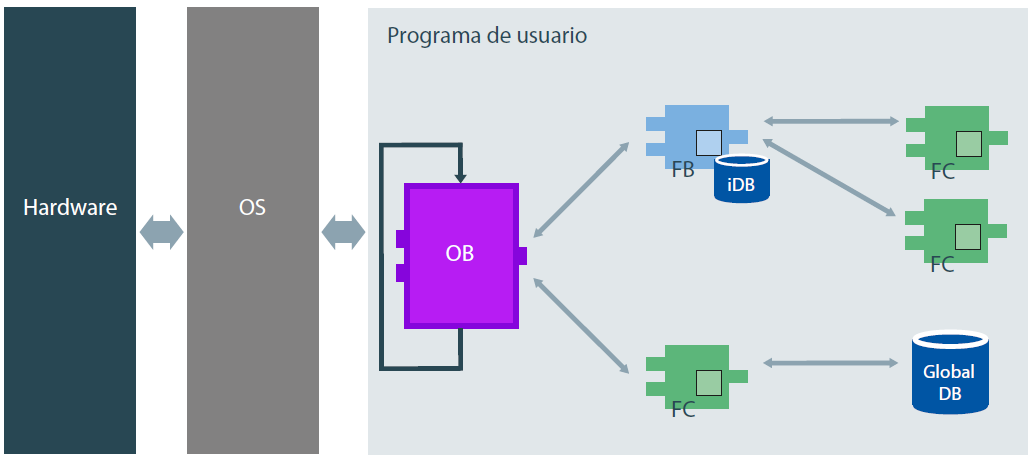
\includegraphics[width=0.85\linewidth]{PLC.png}
	\caption{Programación jerarquizadas en TIA Portal.}
	\label{fig:plc}
\end{figure}


Cada bloque OB, FB o FC puede ser programado con varios lenguajes estandarizados, es decir un FB puede ser programado de cinco formas distintas y también es permitido mesclar distintos lenguajes en la solución jerarquizada. La Figura \ref{fig:languajes} muestra los cinco lenguajes estandarizados por la norma: Diagrama en escalera (LD), Diagrama en Bloque de Funciones (FBD), Lista de Instrucciones (IL), Texto estructurado (ST) y Gráfico de Función Secuencial (SFC). Notese en la Figura \ref{fig:languajes}, que los primeros cuatro lenguajes muestran la respectiva implementación de una AND lógica entre las señales booleanas  S1  y S2. Al respecto SIEMENS nombra dichos lenguajes como: KOP o esquemas de contactos, FUP o diagrama de funciones, AWL o lista de instrucciones, SCL o lenguaje de control estructurado y GRAPH o lenguaje de programación gráfico. La descripción de detallada de cada lenguaje, sus funciones, ejemplos, etc., se encuentran en el manual del sistema \cite{TIA-S7}, para la funcionalidad del KOP incie en página 14161, para el FUP ver página 14223, para  AWL inicia en la página 14283, el SCL se encuentra en la página 14333 y para el GRAPH ver la página 14411.

\begin{figure}
	\centering
	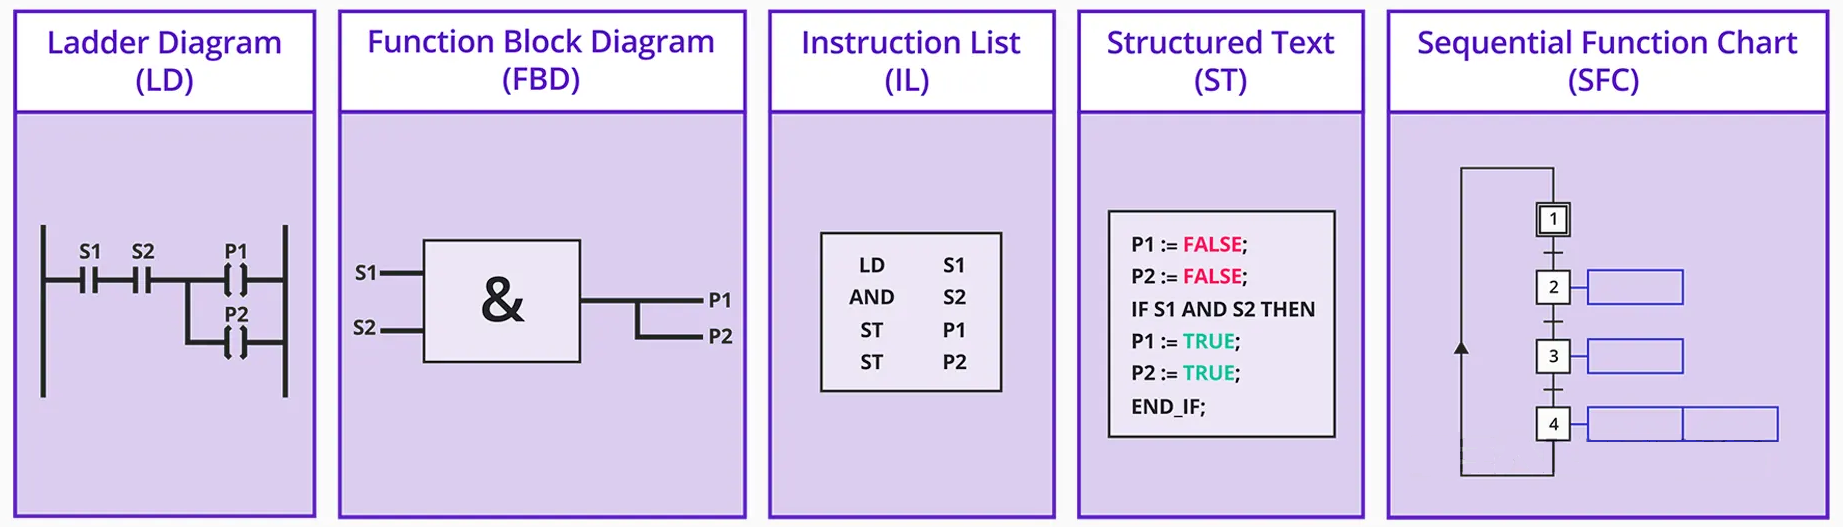
\includegraphics[width=1\linewidth]{Languajes.png}
	\caption{Lenguajes estandarizados por la norma IEC 61131-3.}
	\label{fig:languajes}
\end{figure}


Los diagramas electricos de conexión del CPU S7-1500, de sus módulos de entrada y salida se muestran en el manual del hardware \cite{PLC-1500}. La creación de un proyecto con el Software TIA portal se encuentra en la página  1280 de dicho manual, sin embargo, un video informativo con dicho procedimiento esta disponible en \cite{Maria}. 

\chapter{Repositorio de código}
\label{ap:osc}
\section{Código actividad 1}
\label{ApendiceA1}
{\scriptsize 
    \lstinputlisting[language=Arduino, numbers=none, showstringspaces=false]{L01/A01/A01.ino}
}

\section{Código actividad 2}
\label{ApendiceA2}
{\scriptsize 
    \lstinputlisting[language=Arduino, numbers=none, showstringspaces=false]{L01/A02/A02.ino}
}	

